\hypertarget{group__selectmap__access}{
\section{Selectmap Interface}
\label{group__selectmap__access}\index{Selectmap Interface@{Selectmap Interface}}
}
This module implements the basic access function to the Selectmap interface of the Xilinx FPGA on the RCU.  
\subsection*{API methods: Initialization and general methods.}
\begin{CompactItemize}
\item 
int \hyperlink{group__selectmap__access_g3a82967a2ac2933832a98aa2d822fd7b}{init\-Sm\-Access} (const char $\ast$p\-Device\-Name)
\begin{CompactList}\small\item\em Initialize the interface. \item\end{CompactList}\item 
int \hyperlink{group__selectmap__access_g75466b7556397eb41108eb84212c5b19}{release\-Sm\-Access} ()
\begin{CompactList}\small\item\em Close the device and release internal data structures. \item\end{CompactList}\end{CompactItemize}
\subsection*{Read/write access}
\begin{CompactItemize}
\item 
\_\-\_\-u32 \hyperlink{group__selectmap__access_g88f0784ea00a5707d5fc4db2778e1b2a}{sm\-Make\-T1Header} (\_\-\_\-u8 rdwr, \_\-\_\-u16 address, \_\-\_\-u16 words)
\begin{CompactList}\small\item\em Generates a Type 1 Header Package to send to the selectmap interface. \item\end{CompactList}\item 
int \hyperlink{group__selectmap__access_ge0d7561e2ddca5878fe0c39c948dfdd2}{sm\-Register\-Write} (\_\-\_\-u32 address, \_\-\_\-u32 data)
\begin{CompactList}\small\item\em Write one word to a register of the selectmap interface. \item\end{CompactList}\item 
int \hyperlink{group__selectmap__access_gf7536588344d4c30f928de00a240baa8}{sm\-Register\-Read} (\_\-\_\-u32 address, \_\-\_\-u32 $\ast$p\-Data)
\begin{CompactList}\small\item\em Read one word in a register of the selectmap interface. \item\end{CompactList}\end{CompactItemize}


\subsection{Detailed Description}
This module implements the basic access function to the Selectmap interface of the Xilinx FPGA on the RCU. 



\subsection{Function Documentation}
\hypertarget{group__selectmap__access_g3a82967a2ac2933832a98aa2d822fd7b}{
\index{selectmap_access@{selectmap\_\-access}!initSmAccess@{initSmAccess}}
\index{initSmAccess@{initSmAccess}!selectmap_access@{selectmap\_\-access}}
\subsubsection[initSmAccess]{\setlength{\rightskip}{0pt plus 5cm}int init\-Sm\-Access (const char $\ast$ {\em p\-Device\-Name})}}
\label{group__selectmap__access_g3a82967a2ac2933832a98aa2d822fd7b}


Initialize the interface. 

The device will be opened and some other other internal states initialized. \begin{Desc}
\item[Parameters:]
\begin{description}
\item[{\em p\-Device\-Name,:}]name of the device node, if NULL: /dev/rcu/virtex as default \end{description}
\end{Desc}
\begin{Desc}
\item[Returns:]neg. error code if failed\par
 -ENOSPC : can not get the size of the interface buffers, or buffers too small\par
 -ENOENT : can not open device \end{Desc}


Definition at line 43 of file selectmap\-Interface.c.

References g\_\-p\-Default\-Sm\-Device, and g\_\-Sm\-File.\hypertarget{group__selectmap__access_g75466b7556397eb41108eb84212c5b19}{
\index{selectmap_access@{selectmap\_\-access}!releaseSmAccess@{releaseSmAccess}}
\index{releaseSmAccess@{releaseSmAccess}!selectmap_access@{selectmap\_\-access}}
\subsubsection[releaseSmAccess]{\setlength{\rightskip}{0pt plus 5cm}int release\-Sm\-Access ()}}
\label{group__selectmap__access_g75466b7556397eb41108eb84212c5b19}


Close the device and release internal data structures. 

\begin{Desc}
\item[Returns:]neg. error code if failed \par
 -ENXIO : no device open \end{Desc}


Definition at line 72 of file selectmap\-Interface.c.

References g\_\-Sm\-File.

Referenced by main().\hypertarget{group__selectmap__access_g88f0784ea00a5707d5fc4db2778e1b2a}{
\index{selectmap_access@{selectmap\_\-access}!smMakeT1Header@{smMakeT1Header}}
\index{smMakeT1Header@{smMakeT1Header}!selectmap_access@{selectmap\_\-access}}
\subsubsection[smMakeT1Header]{\setlength{\rightskip}{0pt plus 5cm}\_\-\_\-u32 sm\-Make\-T1Header (\_\-\_\-u8 {\em rdwr}, \_\-\_\-u16 {\em address}, \_\-\_\-u16 {\em words})}}
\label{group__selectmap__access_g88f0784ea00a5707d5fc4db2778e1b2a}


Generates a Type 1 Header Package to send to the selectmap interface. 

\begin{Desc}
\item[Parameters:]
\begin{description}
\item[{\em rdwr}]read (1) or write (0) \item[{\em address}]address of the register \item[{\em words}]of words to read or write (max (2$^\wedge$11)-1) \end{description}
\end{Desc}
\begin{Desc}
\item[Returns:]\end{Desc}


Definition at line 80 of file selectmap\-Interface.c.

Referenced by sm\-Register\-Read(), and sm\-Register\-Write().\hypertarget{group__selectmap__access_gf7536588344d4c30f928de00a240baa8}{
\index{selectmap_access@{selectmap\_\-access}!smRegisterRead@{smRegisterRead}}
\index{smRegisterRead@{smRegisterRead}!selectmap_access@{selectmap\_\-access}}
\subsubsection[smRegisterRead]{\setlength{\rightskip}{0pt plus 5cm}int sm\-Register\-Read (\_\-\_\-u32 {\em address}, \_\-\_\-u32 $\ast$ {\em p\-Data})}}
\label{group__selectmap__access_gf7536588344d4c30f928de00a240baa8}


Read one word in a register of the selectmap interface. 

\begin{Desc}
\item[Parameters:]
\begin{description}
\item[{\em address}]register number \item[{\em p\-Data}]buffer to receive the data \end{description}
\end{Desc}
\begin{Desc}
\item[Returns:]\end{Desc}


Definition at line 148 of file selectmap\-Interface.c.

References g\_\-Sm\-File, SM\_\-REG\_\-READ, sm\-Make\-T1Header(), and VIRTEX\_\-READ\_\-REG.

Referenced by exec\-Read\-Cmd().

Here is the call graph for this function:\begin{figure}[H]
\begin{center}
\leavevmode
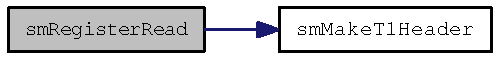
\includegraphics[width=138pt]{group__selectmap__access_gf7536588344d4c30f928de00a240baa8_cgraph}
\end{center}
\end{figure}
\hypertarget{group__selectmap__access_ge0d7561e2ddca5878fe0c39c948dfdd2}{
\index{selectmap_access@{selectmap\_\-access}!smRegisterWrite@{smRegisterWrite}}
\index{smRegisterWrite@{smRegisterWrite}!selectmap_access@{selectmap\_\-access}}
\subsubsection[smRegisterWrite]{\setlength{\rightskip}{0pt plus 5cm}int sm\-Register\-Write (\_\-\_\-u32 {\em address}, \_\-\_\-u32 {\em data})}}
\label{group__selectmap__access_ge0d7561e2ddca5878fe0c39c948dfdd2}


Write one word to a register of the selectmap interface. 

\begin{Desc}
\item[Parameters:]
\begin{description}
\item[{\em address}]register number \item[{\em data}]data word \end{description}
\end{Desc}
\begin{Desc}
\item[Returns:]\end{Desc}


Definition at line 135 of file selectmap\-Interface.c.

References g\_\-Sm\-File, SM\_\-REG\_\-WRITE, sm\-Make\-T1Header(), VIRTEX\_\-SET\_\-REG, and VIRTEX\_\-WRITE\_\-REG.

Referenced by exec\-Write\-Cmd().

Here is the call graph for this function:\begin{figure}[H]
\begin{center}
\leavevmode
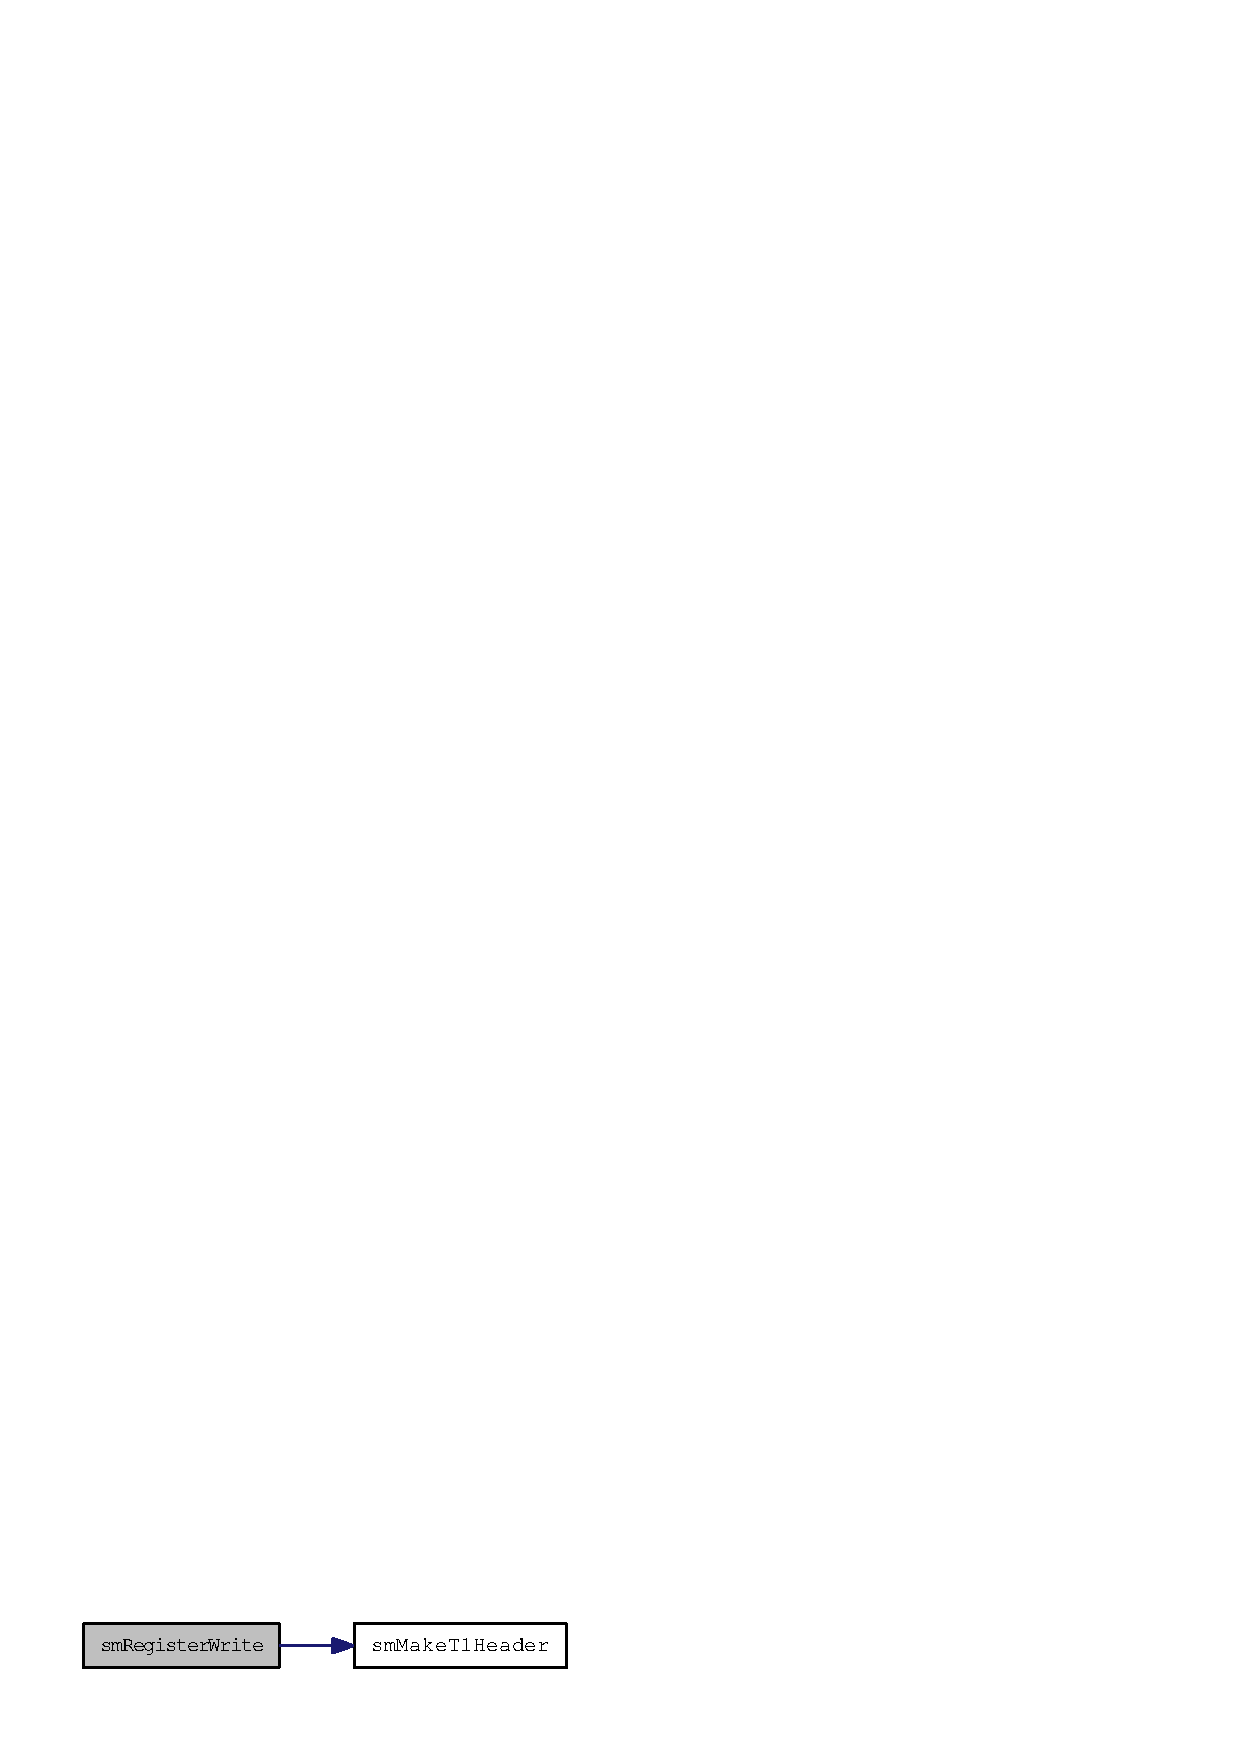
\includegraphics[width=138pt]{group__selectmap__access_ge0d7561e2ddca5878fe0c39c948dfdd2_cgraph}
\end{center}
\end{figure}
